\section{Wechselstromkreise}
\Large 
\begin{frame}
    \centering
    \visible<2->{
    \begin{tikzpicture}
        \path[very thick, -{Latex}] (0, 0) edge (10, 0) (0, -1) edge (0, 3);
        \node[right] at (10, 0) {$t$};
        \draw[thick, red] (0, 0) sin (1, 1) cos (2, 0)
            sin (3, -1) cos (4, 0)
            sin (5, +1) cos (6, 0)
            sin (7, -1) cos (8, 0);
    \end{tikzpicture}
    }
    \\
    \visible<3>{
        \[ A(t) = \hat A\sin(\omega t + \phi) \]
    }
\end{frame}

\section{Die Bauteile}
\begin{frame}{Widerstand}
    \centering\Huge
    \visible<1->{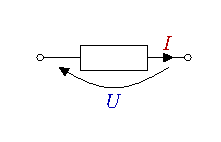
\includegraphics[width=.5\textwidth]{../script/kBR.pdf}}
    \visible<2->{
        $$U = R\cdot I$$
    }
\end{frame}
\begin{frame}{Widerstand}
    \centering\Huge
    \begin{align*}
        U(t) &= R \cdot I(t) \\
        \visible<2->{U(t) &= R \cdot \hat I\sin(\omega t)}
    \end{align*}
    \visible<3>{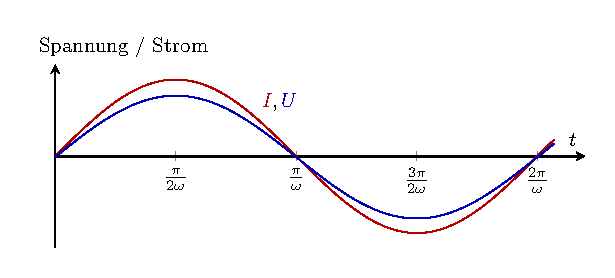
\includegraphics[width=.7\textwidth]{../script/kPR.pdf}}
\end{frame}
\begin{frame}{Kondensator}
    \centering\Huge
    \visible<1->{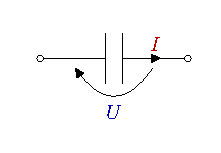
\includegraphics[width=.5\textwidth]{../script/kBC.pdf}}
    \visible<2->{
        \[ I = C\dot U \]
    }
\end{frame}
\begin{frame}{Kondensator}
    \begin{columns}
        \begin{column}{.25\textwidth}
           \begin{align*}
                \visible<1->{I(t) &= C \dv{t} U(t) \\}
                \visible<2->{I(t) &= C \dv{t} \hat U \sin(\omega t - \pi/2) \\}
                \only<-2>{\vphantom{\underbrace{}_{\hat I}}\\}
                \only<3>{I(t) &= \vphantom{\underbrace{}_{\hat I}}
                    \omega C \cdot \hat U \sin(\omega t)\\}
                \only<4->{I(t) &= \underbrace{\omega C \cdot \hat U}_{\hat I} \sin(\omega t)\\}
                \visible<5->{U(t) &= \frac1{\omega C}\cdot\hat I \sin(\omega t - \pi/2)}
            \end{align*}         
        \end{column}
        \begin{column}{.7\textwidth}
            \visible<6>{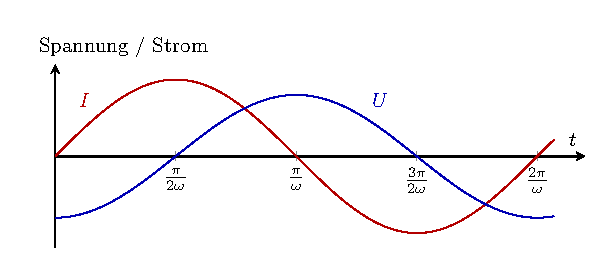
\includegraphics[width=\textwidth]{../script/kPC.pdf}}
        \end{column}
    \end{columns}
\end{frame}
\begin{frame}{Spule}
    \centering\Huge
    \visible<1->{\includegraphics[width=.5\textwidth]{../script/kBL.pdf}}
    \visible<2->{
        \[ U = L\dot I \]
    }
\end{frame}
\begin{frame}{Spule}
    \begin{columns}
        \begin{column}{.25\textwidth}
           \begin{align*}
                \visible<1->{U(t) &= L \dv{t} I(t) \\}
                \visible<2->{U(t) &= L \dv{t} \hat I \sin(\omega t) \\}
                \visible<3->{U(t) &= \omega L \cdot \hat I \sin(\omega t + \pi/2)}
            \end{align*}         
        \end{column}
        \begin{column}{.7\textwidth}
            \visible<3>{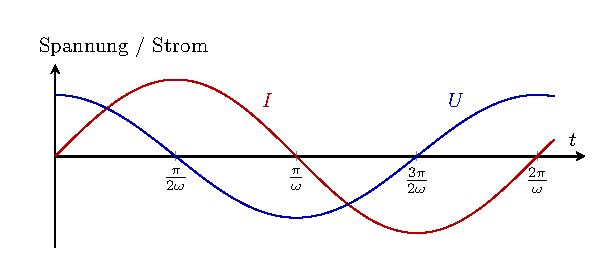
\includegraphics[width=\textwidth]{../script/kPL.pdf}}
        \end{column}
    \end{columns}
\end{frame}
